\documentclass{beamer}
\usepackage[utf8]{inputenc}

\usetheme{Madrid}
\usecolortheme{default}
\usepackage{amsmath,amssymb,amsfonts,amsthm}
\usepackage{txfonts}
\usepackage{tkz-euclide}
\usepackage{listings}
\usepackage{adjustbox}
\usepackage{array}
\usepackage{tabularx}
\usepackage{gvv}
\usepackage{lmodern}
\usepackage{circuitikz}
\usepackage{tikz}
\usepackage{graphicx}

\setbeamertemplate{page number in head/foot}[totalframenumber]

\usepackage{tcolorbox}
\tcbuselibrary{minted,breakable,xparse,skins}



\definecolor{bg}{gray}{0.95}
\DeclareTCBListing{mintedbox}{O{}m!O{}}{%
  breakable=true,
  listing engine=minted,
  listing only,
  minted language=#2,
  minted style=default,
  minted options={%
    linenos,
    gobble=0,
    breaklines=true,
    breakafter=,,
    fontsize=\small,
    numbersep=8pt,
    #1},
  boxsep=0pt,
  left skip=0pt,
  right skip=0pt,
  left=25pt,
  right=0pt,
  top=3pt,
  bottom=3pt,
  arc=5pt,
  leftrule=0pt,
  rightrule=0pt,
  bottomrule=2pt,
  toprule=2pt,
  colback=bg,
  colframe=orange!70,
  enhanced,
  overlay={%
    \begin{tcbclipinterior}
    \fill[orange!20!white] (frame.south west) rectangle ([xshift=20pt]frame.north west);
    \end{tcbclipinterior}},
  #3,
}
\lstset{
    language=C,
    basicstyle=\ttfamily\small,
    keywordstyle=\color{blue},
    stringstyle=\color{orange},
    commentstyle=\color{green!60!black},
    numbers=left,
    numberstyle=\tiny\color{gray},
    breaklines=true,
    showstringspaces=false,
}
%------------------------------------------------------------
%This block of code defines the information to appear in the
%Title page
\title %optional
{4.3.39}
\date{}
%\subtitle{A short story}

\author % (optional)
{Sai Krishna Bakki - EE25BTECH11049}

\begin{document}
\frame{\titlepage}
\begin{frame}{Question}
    If the point (3, 4) lies on the line 3y = ax + 7, find the value of a.
\end{frame}
\begin{frame}{Theoretical Solution}
    Given
\begin{align}
    \vec{P}=\myvec{3\\4},\vec{x}=\myvec{x\\y}\\
    \myvec{a & -3}\vec{x}=-7
\end{align}
Since point (3,4) lies on the line, substitute (1) in (2),we get
\begin{align}
        \myvec{a & -3}\vec{P}=-7\\
        \myvec{a & -3}\myvec{3\\4}=-7\ \\
        3a-12=-7\implies a=\frac{5}{3}
\end{align}
$\therefore$ The value of a is \textbf{$\frac{5}{3}$}.
\end{frame}
\begin{frame}[fragile]
\frametitle{C Code }
\begin{lstlisting}
#include <stdio.h>

// Function to generate points on a line segment between A and B.
// P(lambda) = A + lambda * (B - A)
//
// Parameters:
//   Ax, Ay: Coordinates of the starting point A.
//   Bx, By: Coordinates of the end point B.
//   num_points: The number of points to generate for the line.
//   out_x: A pointer to an array to store the generated x-coordinates.
//   out_y: A pointer to an array to store the generated y-coordinates.
void generate_line_points(double Ax, double Ay, double Bx, double By, int num_points, double* out_x, double* out_y) {
    // Calculate the direction vector m = B - A
    double mx = Bx - Ax;
    double my = By - Ay;
\end{lstlisting}    
\end{frame}
\begin{frame}[fragile]
\frametitle{C Code }
\begin{lstlisting}
    // Generate 'num_points' by varying lambda from 0.0 to 1.0
    for (int i = 0; i < num_points; i++) {
        // Calculate lambda, ensuring it spans from 0 to 1 inclusive
        double lambda = (double)i / (num_points - 1);

        // Calculate the point P using the parametric equation
        // P_x = A_x + lambda * m_x
        // P_y = A_y + lambda * m_y
        out_x[i] = Ax + lambda * mx;
        out_y[i] = Ay + lambda * my;
    }
}
\end{lstlisting}    
\end{frame}
\begin{frame}[fragile]
\frametitle{Python Code Through Shared Output}
\begin{lstlisting}
import ctypes
import numpy as np
import matplotlib.pyplot as plt

# --- 1. Load the Shared C Library ---
# Make sure 'line_generator.so' is in the same directory
try:
    c_lib = ctypes.CDLL('./line.so')
except OSError as e:
    print("Error: Could not load 'line.so'")
    print("Please compile 'line_generator.c' first using:")
    print("gcc -shared -o line_generator.so -fPIC line_generator.c")
    exit()

# --- 2. Define the Python Interface for the C Function ---
# Correctly define the argument types for the C function.
# The last two arguments are pointers to 1D NumPy arrays of doubles.
\end{lstlisting}    
\end{frame}
\begin{frame}[fragile]
\frametitle{Python Code Through Shared Output}
\begin{lstlisting}
c_lib.generate_line_points.argtypes = [
    ctypes.c_double, ctypes.c_double,
    ctypes.c_double, ctypes.c_double,
    ctypes.c_int,
    np.ctypeslib.ndpointer(dtype=np.double, ndim=1, flags='C_CONTIGUOUS'),
    np.ctypeslib.ndpointer(dtype=np.double, ndim=1, flags='C_CONTIGUOUS')
]
c_lib.generate_line_points.restype = None


# --- 3. Prepare Data for the Line and Point ---
# The line is 3y = (5/3)x + 7  or y = (5/9)x + 7/3

# To use our C function, we find two points on the line.
# Let's pick x = -12 and x = 5 to get a good range.
x1 = -12.5
\end{lstlisting}    
\end{frame}
\begin{frame}[fragile]
\frametitle{Python Code Through Shared Output}
\begin{lstlisting}
y1 = (5/9)*x1 + (7/3)
A = np.array([x1, y1])

x2 = 5.0
y2 = (5/9)*x2 + (7/3)
B = np.array([x2, y2])

# This is the specific point we want to show on the line
P = np.array([3.0, 4.0])

num_points = 100 # Number of points to make the line smooth

# Create empty NumPy arrays to be filled by the C function
line_x = np.zeros(num_points, dtype=np.double)
line_y = np.zeros(num_points, dtype=np.double)

\end{lstlisting}    
\end{frame}
\begin{frame}[fragile]
\frametitle{Python Code Through Shared Output}
\begin{lstlisting}
# --- 4. Call the C Function ---
c_lib.generate_line_points(
    A[0], A[1],       # Start point A
    B[0], B[1],       # End point B
    num_points,
    line_x,           # Output array for x-coords
    line_y            # Output array for y-coords
)

# --- 5. Plot the Results ---
plt.figure(figsize=(8, 6))

# Plot the line generated by the C code
a = 5/3
plt.plot(line_x, line_y, label=f'Line 3y = ({a:.2f})x + 7')

# Plot the specific point, ensuring coordinates are Python ints for the label
\end{lstlisting}    
\end{frame}
\begin{frame}[fragile]
\frametitle{Python Code Through Shared Output}
\begin{lstlisting}
plt.plot(P[0], P[1], 'ro', markersize=8, label=f'Point {tuple(map(int, P))}')

# Add styling to match the example image
plt.title("Verification Plot")
plt.xlabel("X-axis")
plt.ylabel("Y-axis")
plt.grid(True)
plt.legend()
plt.axis('equal')
plt.show()
\end{lstlisting}    
\end{frame}
\begin{frame}[fragile]
\frametitle{Python Code}
\begin{lstlisting}
import numpy as np
import matplotlib.pyplot as plt
from libs.funcs import line_norm # Import the required function

# The value of 'a' we calculated
a = 5/3

# Line equation: 3y = (5/3)x + 7
# Standard form: 5x - 9y + 21 = 0
# This is in the form n.T @ x + k = 0
# The normal vector n is [5, -9]
# The constant term is 21, so n.T @ x = -21
\end{lstlisting}    
\end{frame}
\begin{frame}[fragile]
\frametitle{Python Code}
\begin{lstlisting}
# 1. Define the line's properties for the plotting function
n = np.array([5, -9]).reshape(-1, 1)
c = -21

# 2. Generate the coordinate data for the line

# We use a large range (-10, 10) to ensure the line is long enough for the plot
line_coords = line_norm(n, c, -10, 10)

# 3. Define the point that lies on the line
P = np.array([3, 4])

# 4. Plot the results
plt.plot(line_coords[0, :], line_coords[1, :], label=f'Line 3y = ({a:.2f})x + 7')
plt.plot(P[0], P[1], 'ro', label='Point (3, 4)') # 'ro' for red circle
\end{lstlisting}    
\end{frame}
\begin{frame}[fragile]
\frametitle{Python Code}
\begin{lstlisting}
# Add labels and a grid for better visualization
plt.xlabel("X-axis")
plt.ylabel("Y-axis")
plt.title("Verification Plot")
plt.grid(True)
plt.legend()
plt.axis('equal') # Ensures correct aspect ratio

# Display the plot
plt.show()
\end{lstlisting}
\end{frame}
\begin{frame}{Plot By C code and Python Code}
    \begin{figure}
    \centering
    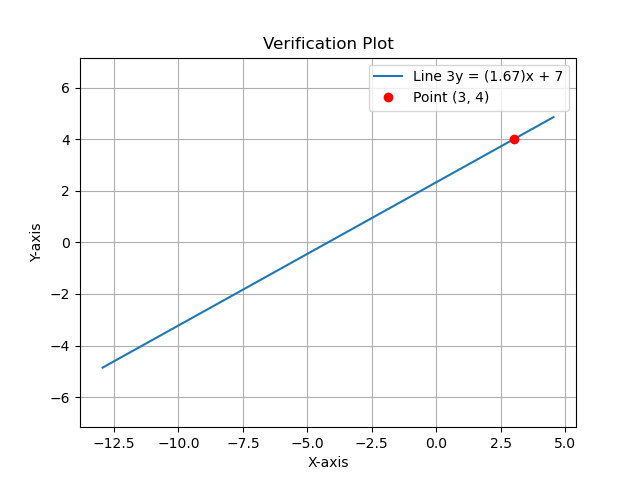
\includegraphics[width=0.7\columnwidth]{figs/Figure_1.png}
    \label{fig:placeholder}
    \caption{1}
\end{figure}
\end{frame}
\end{document}